%
% sekanten.tex
%
% (c) 2020 Prof Dr Andreas Müller, Hochschule Rapperwil
%
\begin{frame}
\frametitle{Sekantenverfahren}
\vspace{-10pt}
\begin{columns}[t]
\begin{column}{0.48\hsize}
\begin{block}{Strahlensatz}
\vspace{-15pt}
\begin{align*}
(a-x_0) : f(a) &= (b-x_0) : f(b)
\\
\uncover<2->{af(b) -x_0f(b)}&\uncover<2->{= bf(a)-x_0f(a)}
\\
\uncover<3->{x_0}&\uncover<3->{=\frac{af(b)-bf(a)}{f(b)-f(a)}}
\end{align*}
\vspace{-15pt}
\end{block}
\uncover<4->{
\begin{block}{Iteration}
\vspace{-15pt}
\[
x_{n+1}
=
\frac{f(x_n)x_{n-1}-f(x_{n-1})x_n}{f(x_n)-f(x_{n-1})}
\]
\uncover<5->{%
Lineare Konvergenz:
\[
\lim_{n\to\infty} x_n = x^*,\quad f(x^*)=0
\]}
\end{block}}
\end{column}
\begin{column}{0.48\hsize}
\begin{center}
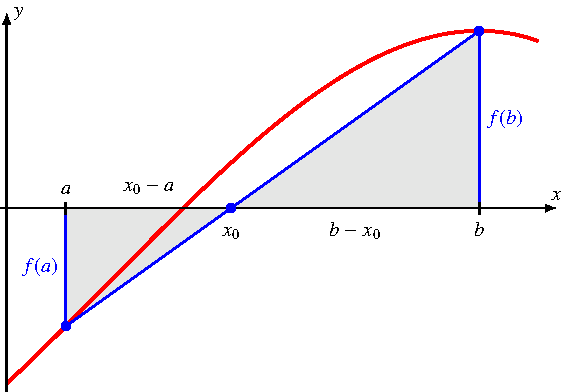
\includegraphics[width=\hsize]{../../buch/chapters/20-gleichungen/figures/sekante.pdf}
\end{center}
\uncover<6->{%
\begin{block}{Probleme}
\begin{itemize}
\item<7-> Auslöschung
\item<8-> langsame Konvergenz
\end{itemize}
\end{block}}
\end{column}
\end{columns}
\end{frame}
